\section{Úvod}
\label{sec:Úvod}

Matematické kyvadlo je nejjednodušším typem kyvadla. Máme hmotný bod o hmotnosti $m$ zavěšený na provázku délky $l$ zanedbatelné hmotnosti. Tření a odpor vzduchu nezapočítáváme. Tíhové pole považujeme za homogenní s tíhovým zrychlením $g$.

\section{Pohybová rovnice}
\label{sec:Pohybová rovnice}
Teď se podíváme na pohybovou rovnici. Hmotný bod se pohybuje po kružnici o poloměru $l$ a jeho pohyb popisujeme aktuálním úhlem $\varphi(t)$, který měří výchylku z dolní rovnovážné polohy. Pro zrychlení platí $a=l\varepsilon=l\dot{\omega}=l\ddot{\varphi}$ a pro vratnou sílu platí $F=-mg\sin\varphi$. Teď použijeme 2. Newtonův zákon: $F=ma$.
\begin{equation*}
ma=ml\ddot{\varphi}=F=-mg\sin\varphi\\
\end{equation*}
Můžeme pokrátit $m$ z naší rovnice a vydělíme celou rovnici $l$. Pak vše převedeme na jednu stranu. Dostáváme pohybovou rovnici matematického kyvadla.
\begin{equation}
\boxed{\ddot{\varphi}+\frac{g}{l}\sin\varphi=0}
\end{equation}
Vidíme, že naše rovnice je nelineární diferenciální rovnice druhého řádu. Pokud budeme brát v úvahu jen malé výchylky z rovnovážné polohy, můžeme rovnici linearizovat.
\begin{equation}
\ddot{\varphi}+\frac{g}{l}\varphi=0
\end{equation}
Využili jsme Taylorova rozvoje $\sin\varphi$:
\begin{equation*}
\sin\varphi = \varphi-\frac{\varphi^3}{6}+\frac{\varphi^5}{120}+O\left(\varphi^6\right)
\end{equation*}
Kde jsme vzali jen první člen, neboť nás zajímají jen malé výchylky.

\section{Ladíkova sekce}
\label{sec:Ladíkova sekce}

Traalalalal

\begin{figure}[h]
  \centering
  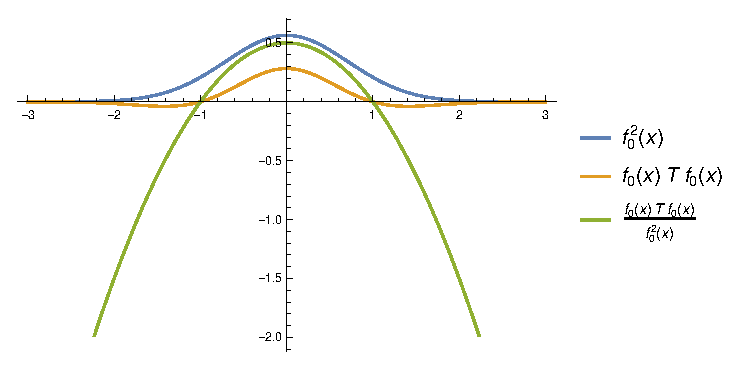
\includegraphics[width=0.6\textwidth]{figures/1.eps}
  \caption{Cycloid.}
  \label{fig:pendulum-cycloid}
\end{figure}

%%% Local Variables:
%%% mode: latex
%%% TeX-master: "../pendulum"
%%% End:
